\chapter{Présentation générale}



\section{Présentation du projet}
Aujourd'hui, détecter les points des articulations du corps humain 
est une technique courante, grâce à certain périphérique tel que la 
Kinect. Les points des articulations du corps forment le squelette 3D. 
Cependant, les squelettes 3D sont en générales pas assez riche en 
informations concernant les points des articulations des mains.\\

Pourtant les mains sont habiles et nous pouvons faire de nombreux 
mouvements, plus ou moins complexes et rapides avec elles. De plus en 
plus d'applications nécessitent des IHM plus précisent et plus 
naturelles. Utiliser ces mains pour contrôler, interagir et communiquer 
avec un ordinateur, devient très intéressant. Ce niveau de 
précision peut être utile dans divers domaines :
\begin{itemize}
  \item simulation médicale.
  \item modélisation et CAO\footnote{Conception Assisté par Ordinateur}.
  \item manipulation d'objets 3D virtuels.
  \item jeux vidéo.\\
\end{itemize}

Le projet \og Hand Kinect \fg consiste à extraire depuis une Kinect 2, 
les points correspondants aux articulations du corps grâce aux 
fonctions du SDK de ce capteur. De plus, nous devons récupérer les points 
des articulations des mains, pour cela nous étudions plusieurs méthodes 
réalisées jusqu'à maintenant. Ainsi, l'assemblage de ces points nous 
permet d'obtenir le squelette 3D complet de la personne devant la 
Kinect.\\

\begin{figure}[H]
  \begin{center}
    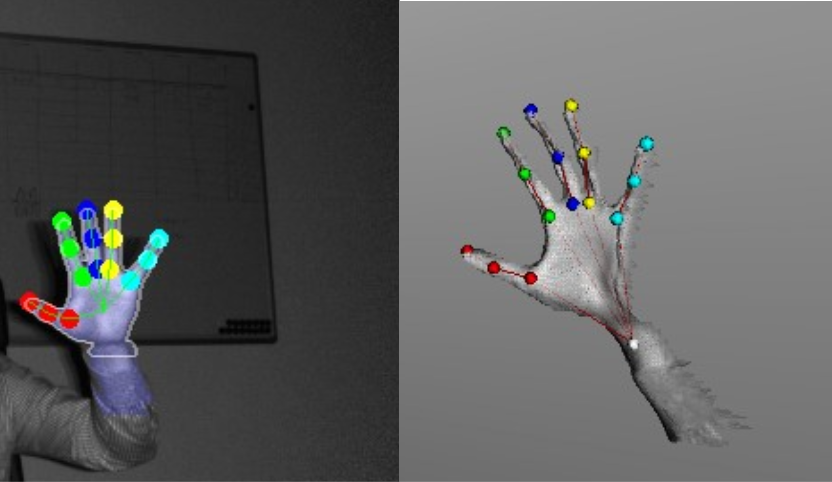
\includegraphics[width=350px]{images/joint_detection.png}
    \caption{Détection des articulations des mains}
  \end{center}
\end{figure}

Ensuite, nous souhaitons animer un modèle 3D, qui peut être un modèle 
d'humain, de robot ou bien de créature. Les mouvements de ce modèle 
doivent suivre les points du squelette préalablement détectés, de 
manière cohérente par rapport aux mouvements de la personne devant la 
Kinect. Nous utilisons Unity3D, pour cette partie de 
modélisation.\\

Unity3D est un moteur de jeu qui permet de développer rapidement des 
environnement et application 3D. Il est facile d'obtenir des 
applications compatibles sur de nombreuses plateformes. Ce moteur 
propose également une licence gratuit assez complète.\\

\begin{figure}[H]
  \begin{center}
    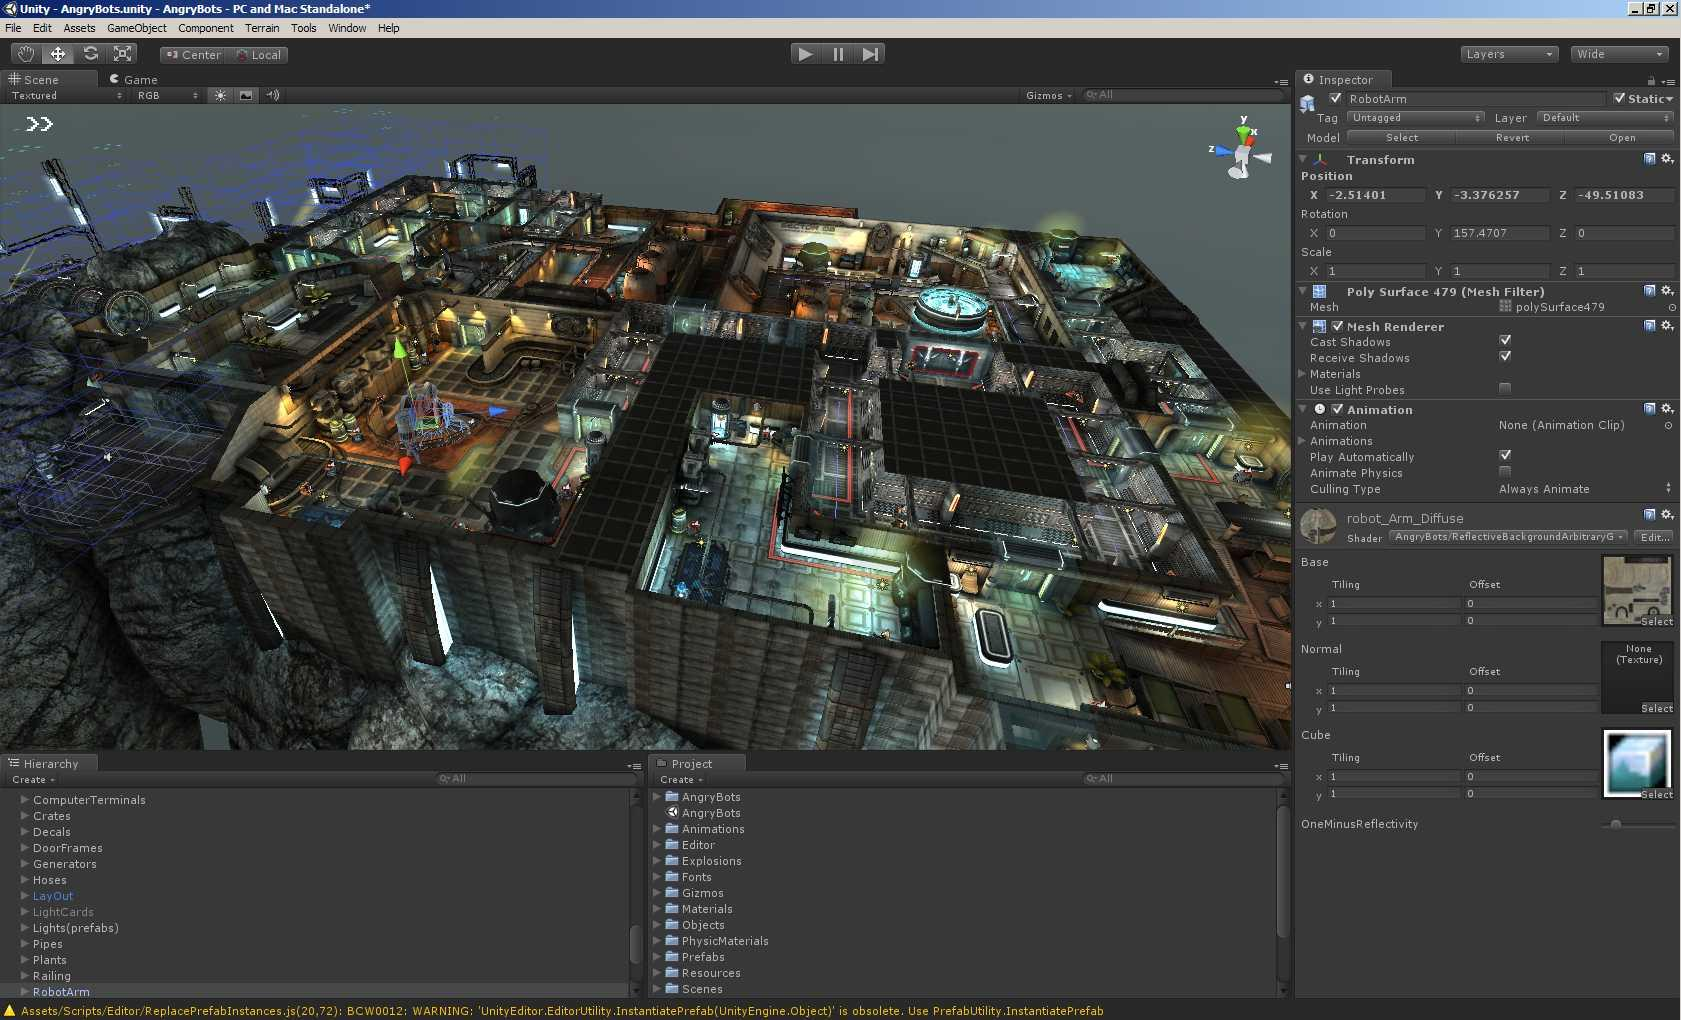
\includegraphics[width=350px]{images/Unity3D.jpg}
    \caption{Interface de Unity3D}
  \end{center}
\end{figure}

Dans le cadre de ce projet, nous sommes amenés à rédiger un état de la 
l'art. Cette première partie, nous permet de synthétiser et sélectionner 
les solutions. Notre objectif étant de détecter la main d'une personne 
et ses articulations, afin de modéliser en 3D la main de 
cette personne, dans des plans de caméra global ou rapprocher. Cela 
doit être réalisable en temps réel et à partir d'une caméra nous 
fournissant une image RGB et une image contenant l'information de 
profondeur de la scène filmée.\\

\section{Contexte}
La réalisation de ce projet se fait avec l'équipe 3D 
SAM\footnote{Modeling and Analysis of Static and Dynamic Shapes}. 
Cette équipe appartient au centre CRIStAL\footnote{Centre de Recherche 
en Informatique, Signal et Automatique de Lille}. Ce centre est le 
nouveau pôle de recherche qui regroupe les laboratoires d'informatique, 
signal et automatique de Lille.\\

L'équipe 3D SAM est basée à l'école d'ingénieur Télécom Lille 1. 
Cette équipe conçoit de nouveaux outils et méthodes d'analyse des 
formes des objets 3D statiques et dynamique. Ils travaillent sur 
l'analyse de formes des objets 3D et la modélisation des variations 
des formes dans des vidéos 3D.

\begin{figure}[H]
  \begin{center}
    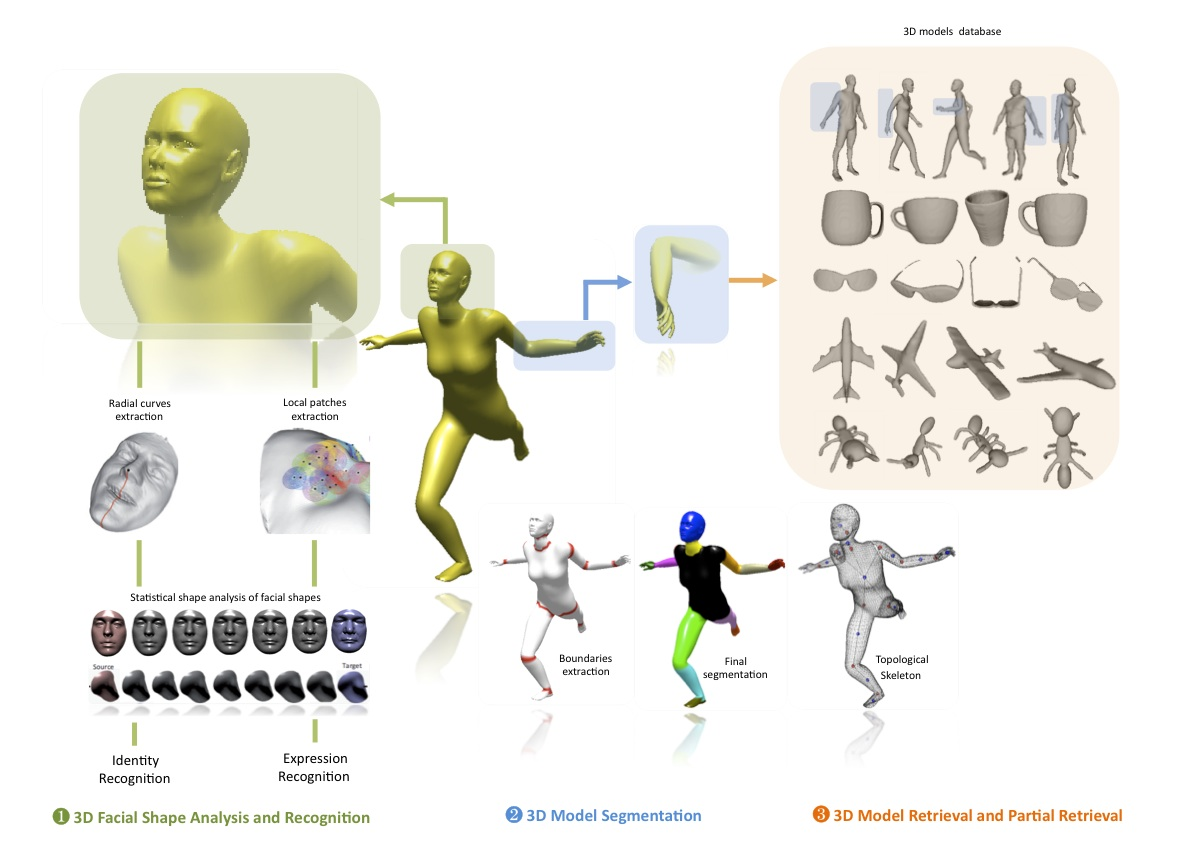
\includegraphics[width=300px]{images/accueil-illus.jpg}
    \caption{Exemples de travaux de l'équipe 3D SAM}
  \end{center}
\end{figure}

%TODO pour le module -> vu l'état de l'art on considere qu'on la pas tout de suite
Le projet \og Hand Kinect \fg est un nouveau projet proposé par 
l'équipe.
Pour sa réalisation, nous disposons d'une caméra Kinect 2. 
Pour les représentations et animations 3D, il nous faut un environnement 
de modélisation. Nous utilisons Unity3D comme montré précédemment. 
Nous disposons également, d'un module nous permettant d'extraire les 
points des articulations de la main.

\section{Problèmatique}
D'abord, la Kinect 2 peux déjà suivre six personnes à la fois. Elle 
détecte un squelette de vingt-six points (voir Fig. 
\ref{fig:skeleton_kinect2} et \ref{fig:kinect1vs2}). Cependant, les 
mains ne sont représentées seulement par trois points, qui sont le 
centre de main, le pouce et le bout du majeur. C'est une amélioration 
par rapport à la Kinect 1, qui ne détectait que le centre de la main.\\

D'autre outils permettent de détecter les mains des utilisateurs. Par 
exemple le Leap Motion détecte les articulations des mains. Néanmoins,
ce capteur est limité, car il faut garder les mains proches et dans le 
cadre du capture. Leap Motion ne permet pas de détecter le squelette 
complet d'une personne.\\

À partir de ces constats nous pouvons formuler la problématique 
suivante. Puisque, 
les mains sont très habiles, il peut être difficile de détecter leurs 
articulations dans des positions contraignantes. En supplément, les 
problèmes liés à la luminosité sont récurrents, il est souhaitable 
d'utiliser des techniques robustes et invariantes à la luminosité, 
mais qui restent efficaces. De plus, il existe encore peu de méthodes 
permettant de détecter la pose et les articulations des mains dans 
un point de vue de caméra qui permettrais de retrouver l'ensemble du
squelette humain.

%comment réaliser ce projet, avec quoi + résultat attendu
\section{Objectif}
%TODO objectif de l'état de l'art
%Le premier objectif est la détection des points des articulations 
%des mains. Pour cela, nous utilisons le module fournit par nos 
%tuteurs. Ainsi, il faut extraire les points des articulation des 
%mains, afin de les rendre utilisable dans Unity3D.\\
%
%En suite, un second objectif consiste modéliser les points des 
%articulations des mains, dans le but d'obtenir une première 
%visualisation simple. Il faut également pouvoir récupérer le 
%squelette calculer par la Kinect 2.\\
%
%Le troisième objectif est de déterminer quelque type de modèle 3D, 
%nous allons utiliser avec de représenter la main. Et, déterminer 
%si il faut segmenter les modèles de mains pour notre application.\\
%
%Après cela, le quatrième objectif est de faire correspondre un 
%modèle 3D de main avec les points des articulations détectés. Un 
%script C\# pour Unity3D peut permettre d'effectuer cette 
%correspondance.\\
%
%Enfin le dernier objectif est de rassembler les points des articulations 
%des mains détecté et les points du squelette calculés par la Kinect 2. 
%Afin de animer un personnage virtuel 3D dont les mouvements sont guidés 
%par les gestes de l'utilisateur devant la Kinect 2. 

L'objectif de cette première partie du projet est de clarifier nos 
travaux. Pour cela, \ldots


\section{Présentation de la Kinect 2}
La Kinect 2 de Microsoft possède une caméra couleur en mode YUV de 1920x1080 pixel.
YUV est une combination particulière d'information pour restituer la couleur, comme RGB ou HSP.
Cette combinaison aussi appelée YCbCr, avec Y la luminance, U/Cb la composante bleu sans luminance et V/Cr la composante rouge sans luminance
En plus de sa caméra, elle possède 3 diffuseur de rayonnement infrarouges qui servent à dessiner une carte de profondeur.
Les autres fonctionnalités ne nous intéresseront pas résoudre notre problèmatique.\\

\begin{figure}[H]
 \center
 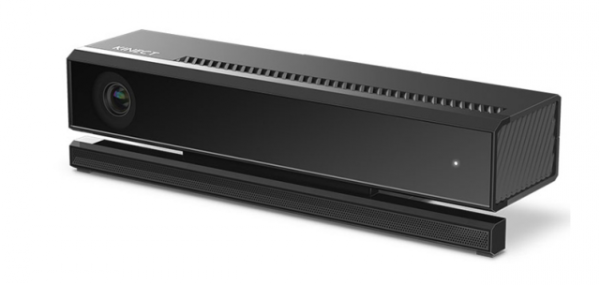
\includegraphics[width=300px]{images/kinect-v2.png}
 \caption{Caméra Kinect 2}
\end{figure}

On récupère donc de Kinect les données brutes suivantes : 
\begin{itemize}
 \item un flux vidéo couleur en YUV
 \item un flux vidéo d'images de profondeur
\end{itemize}

Ces deux flux peuvent servir à détecter la main (méthodes expliquées dans la partie état de l'art).
Le SDK de la Kinect fournit des informations déjà traitées. 
Par exemple pour notre projet, les jointures du poignet, du centre de la main, du sommet du pouce et du sommet du majeur.

\begin{figure}[H]
\center
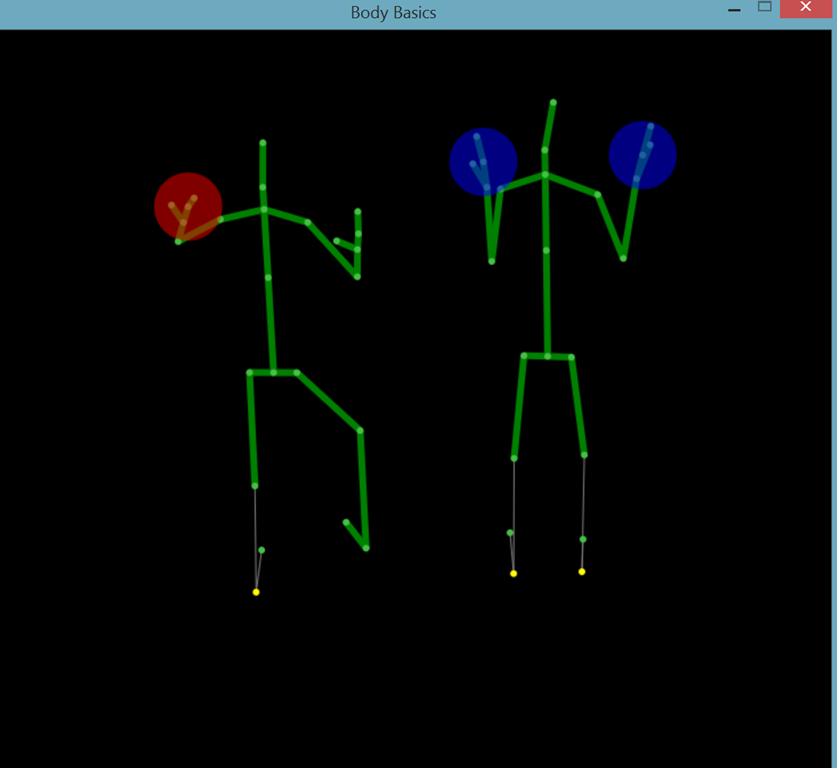
\includegraphics[width=250px]{images/kinec2_skel.png}
\caption{Squelette de l'utilisateur détecté par la Kinect 2}
\label{fig:skeleton_kinect2}
\end{figure}

\begin{figure}
  \begin{center}
    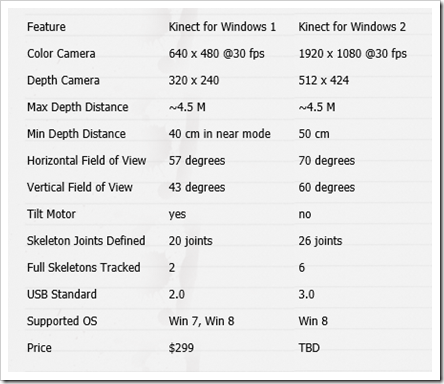
\includegraphics[width=250px]{images/Kinect1vs2.png}
    \caption{Différence Kinect 1 et Kinect 2}
    \label{fig:kinect1vs2}
  \end{center}
\end{figure}

%présentation du materiel + image materiel
%présentation des données brut
%présentation du sdk + image squelette
